\documentclass{article}


\usepackage[english]{babel}
\usepackage[applemac]{inputenc}
\usepackage{graphicx}
\usepackage{geometry}
\usepackage{float}
\usepackage{moreverb}

\newfloat{screenshot}{}


\title{TLACE Visualizer --- User Manual}
\author{Simon Busard}


\begin{document}

	\maketitle
	
	% Intro
	TLACE Visualizer is a tree-like annotated counter-examples (TLACEs) visualizer and browser. It displays TLACEs in a graph structure and allows their browsing.
	This manual gives a brief description of the tool, its usage and features. It assumes that TLACE Visualizer is compiled and launched.
	
	% Screenshot
	\begin{screenshot}[!ht]
		\centering
		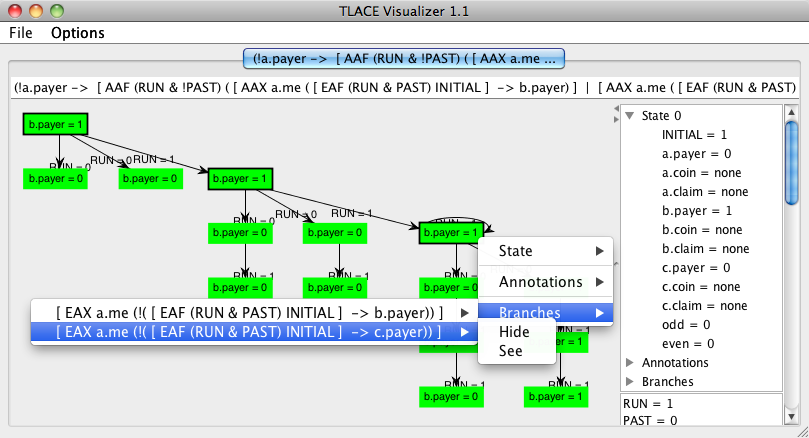
\includegraphics[width=\textwidth]{images/Screenshot.png}
	\end{screenshot}
	
	% How-to --- features
	\section*{How-to}
	
	The input format supported by TLACE Visualizer is given by the grammar at the end of this manual. This format is an XML format containing tree-like annotated counter-examples. Several counter-examples can be imported in TLACE Visualizer and accessed through to the tabulations at the top of the tool.
	
	When imported, the counter-example is displayed in a graph structure where each vertex is a node of the counter-example and each edge a transition. The graph is laid out using a custom layout designed to keep the structure of the counter-example, displaying vertical main path and oblique branches.  Parts of the graph can be rearranged by drag-and-drop.
	
	Nodes information can be accessed by popup menus (right-clicking on the corresponding vertex). This popup menu displays the values of state variables of the model in the state of the node. It also gives its annotation and the list of branches. Each branch can be inspected as a path or fold/unfold through this menu. When a branch is fold, it disappears of the graph with its sub-branches. It can be unfolded again through the same menu.
	
	The tool allows also to inspect a particular path in the graph. To do so, select a node with CTRL pressed (or CMD for Mac OSX) and then select another node. If there is a path in the graph from the first node to the second one, a side panel is opened and displays the information of all nodes of the path.
	
	% Options
	\section*{Options}
	
	The tool has several options. Some options are common to imported counter-examples and located in the top-level menu bar.
	\begin{itemize}
		\item \texttt{Set default layout} sets the layout used for future imported counter-examples.
		\item \texttt{Set default info panel} sets the way the path information are given.
		\item \texttt{Open counter-examples fully folded} asks the tool to display imported counter-examples as a single initial node from which branches can be unfolded manually.
	\end{itemize}
	Other options are particular to each imported counter-example and located in the tabulations.
	\begin{itemize}
		\item \texttt{Set layout} changes the layout of the graph.
		\item \texttt{Set info panel} sets the way the path information are given for this counter-example.
		\item \texttt{Display values on the graph} allows the user to choose which state and input variables are displayed on the graph, in the nodes and on the transitions, respectively.
		\item \texttt{Show only changed variables}, when activated, displays only variables which value changes from the previous state in the list of nodes of the path description.
	\end{itemize}
	
	
	% XML format
	\newpage
	\section*{XML Format}
	
	\begin{verbatimtab}[4]
XML			::=	<?xml version="1.0" encoding="UTF-8"?>
					CNTEX
CNTEX		::=	<counterexample specification="SPEC">
					NODE
				</counterexample>
NODE		::=	<node id="ID">
					STATE
					ATOMIC*
					EXISTENTIAL*
					UNIVERSAL*
				</node>
STATE		::=	<state>
					VALUE+
				</state>
VALUE		::=	<value variable="NAME">VAL</value>
ATOMIC		::=	<atomic specification="SPEC" />
EXISTENTIAL	::=	<existential specification="SPEC" explained="true">
					PATH
				</existential>
				| <existential specification="SPEC" explained="false" />
UNIVERSAL	::=	<universal specification="SPEC" />
PATH		::=NODE (INPUT NODE)+ LOOP?
INPUT		::=<combinatorial>
					VALUES*
				</combinatorial>
				<input>
					VALUES*
				</input>
LOOP		::=	INPUT
				<loop to="ID" />
	\end{verbatimtab}

\end{document}